\documentclass[12pt, a4paper]{article}
\usepackage[utf8]{inputenc}
\usepackage{physics}
\usepackage{graphicx}
\usepackage{amsmath}
\usepackage{cancel}
%code color
\usepackage{listings}
\usepackage{xcolor}

\definecolor{codegreen}{rgb}{0,0.6,0}
\definecolor{codegray}{rgb}{0.5,0.5,0.5}
\definecolor{codepurple}{rgb}{0.58,0,0.82}
\definecolor{backcolour}{rgb}{0.95,0.95,0.92}

\lstdefinestyle{mystyle}{
	backgroundcolor=\color{backcolour},   
	commentstyle=\color{codegreen},
	keywordstyle=\color{magenta},
	numberstyle=\tiny\color{codegray},
	stringstyle=\color{codepurple},
	basicstyle=\ttfamily\footnotesize,
	breakatwhitespace=false,         
	breaklines=true,                 
	captionpos=b,                    
	keepspaces=true,                 
	numbers=left,                    
	numbersep=5pt,                  
	showspaces=false,                
	showstringspaces=false,
	showtabs=false,                  
	tabsize=2
}

\lstset{style=mystyle}

\begin{document}
	\begin{center}
		Test 2  Entanglement
	\end{center}
	
	Mr. Phiphat Chomchit 630631028
	\begin{enumerate}
		\item Suppose you have 5 qubits in the state  $\ket{\Psi} = \frac{1}{\sqrt{2}}\ket{01010} + \frac{1}{\sqrt{2}}\ket{10101} .$ Is state $\ket{\Psi}$ entangled? Why?\\
		
		Ans:
		\begin{itemize}
			\item Measurement results of entangled qubits are correlated.
			$$\ket{B_{00000} } =  \frac{1}{\sqrt{2}}\ket{01010} + \frac{1}{\sqrt{2}}\ket{10101} \implies 
			\begin{cases}
				P(0) =  \left|\frac{1}{\sqrt{2}}\right|^2 = \frac{1}{2}\\
				P(1) =  \left|\frac{1}{\sqrt{2}}\right|^2 = \frac{1}{2}
			\end{cases}
			$$
			
			if we measure first qubit and get outcome 0. Calculate the post-measurement state of the qubit pair by removing the term which is no-consistent with the measurement result.
			$$\ket{B_{00000} } = \frac{1}{\sqrt{2}}\ket{01010} + \cancel{\frac{1}{\sqrt{2}}\ket{10101}} \implies \frac{\frac{1}{\sqrt{2}}\ket{01010}}{\sqrt{\left|\frac{1}{\sqrt{2}}\right|^2}} = \ket{01010}$$
			\item Partial and simultaneous measurements give the same outcome.
			
			\begin{align}
				P(01010) &= \left|\frac{1}{\sqrt{2}}\right|^2 = \frac{1}{2}\\
				P(10101) &= \left|\frac{1}{\sqrt{2}}\right|^2 = \frac{1}{2}
			\end{align}
			\item The state of the entangled qubits cannot be written as the product of the signle-qubit states.
			
			Proof by contradiction.\\
			Let $\ket{\Psi}$ can be written as the product of the single-qubit states and
			$$\ket{S_i} = a_i\ket{0} + b_i\ket{1}$$
			for $i = 1, 2, 3, 4, 5$\\
			So, the product of single-qubit states is
			$$\ket{S} = \ket{S_1}\ket{S_2}\ket{S_3}\ket{S_4}\ket{S_5}$$
			
			From "$\ket{\Psi}$ can be written as the product of the single-qubit states". So
			
			\begin{align}
				\ket{\Psi} &= \ket{S}\\
				 \frac{1}{\sqrt{2}}\ket{01010} + \frac{1}{\sqrt{2}}\ket{10101} &= \ket{S}
			\end{align}
			This implies $a_1b_2a_3b_4a_5 = b_1a_2b_3a_4b_5 = \frac{1}{\sqrt{2}}$, otherwise $0$.\\
			Consider $a_1a_2a_3a_4a_5 = 0$ That is $a_i = 0$ for some $i \in \{1,2,3,4,5\}$
			case: $a_i = 0$ when $i$ is odd number. Then $a_1b_2a_3b_4a_5 = 0$.\\
			case: $a_i = 0$ when $i$ is even number. Then $b_1a_2b_3a_4b_5 = 0$.\\
			Contradiction, therefore $\ket{\Psi}$ cannot be written as the product of the single-qubit states
		\end{itemize}

		\item Write a program to generate $\ket{\Psi}$, run it 1024 times, and come up with an example how to use it in quantum communication.
		\begin{lstlisting}[language=Python, caption=IBM Q code]
			OPENQASM 2.0;
			include "qelib1.inc";
			
			qreg q[5];
			creg c[5];
			
			h q[0];
			x q[1];
			x q[3];
			cx q[0],q[1];
			cx q[0],q[2];
			cx q[0],q[3];
			cx q[0],q[4];
			measure q[0] -> c[0];
			measure q[1] -> c[1];
			measure q[2] -> c[2];
			measure q[3] -> c[3];
			measure q[4] -> c[4];
		\end{lstlisting}
	
			\begin{figure}
				 \centering
				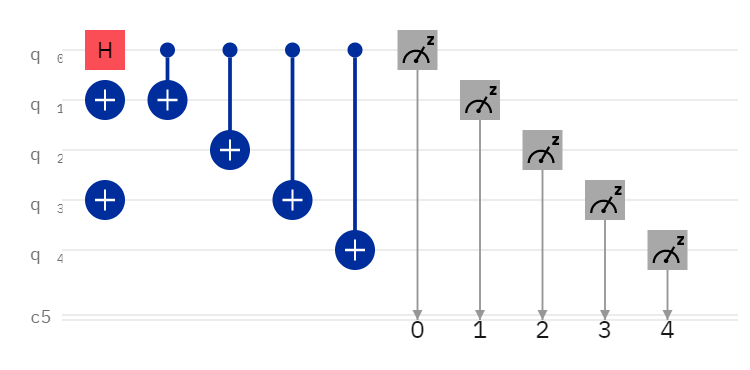
\includegraphics[scale=0.3]{circuit-krik226j.png}
				\caption{quantum circuit}
				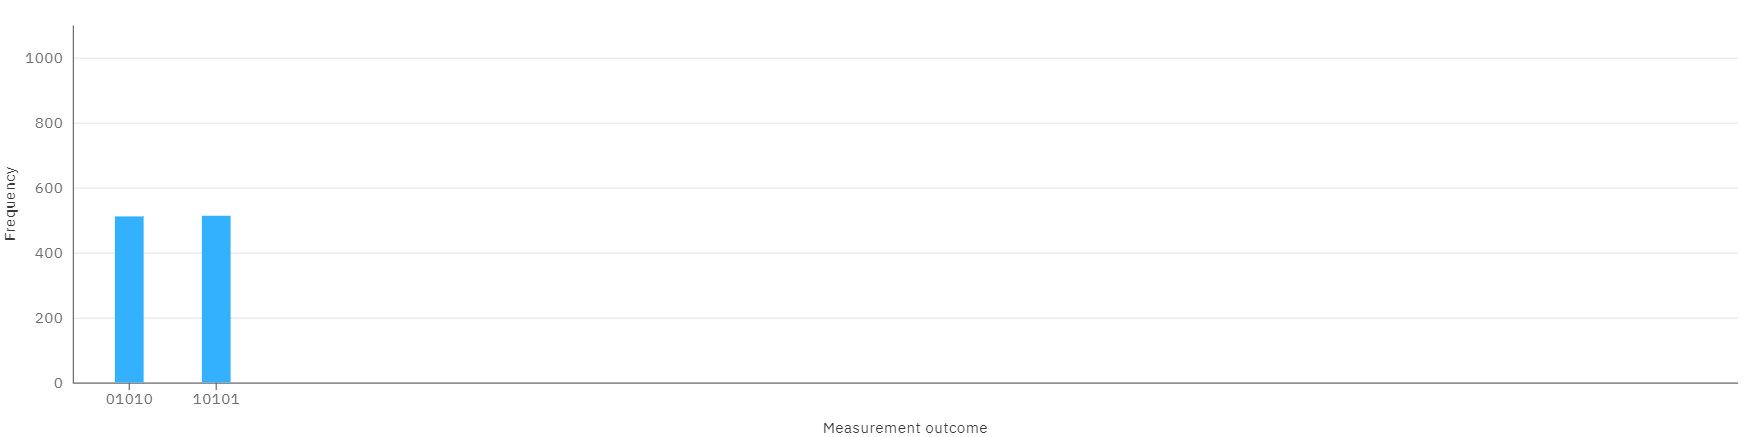
\includegraphics[scale=0.2]{bar-chart.png}
				\caption{result}
			\end{figure}

		
	\end{enumerate}
\end{document}